%!TEX root = ./template-skripsi.tex
%-------------------------------------------------------------------------------
%                            BAB II
%               KAJIAN TEORI
%-------------------------------------------------------------------------------

\chapter{KAJIAN TEORI}                

\section{Sistem Informasi Manajemen}
	\subsection{Sistem}
	Sistem berasal dari bahasa latin (\emph{systēma}) dan bahasa Yunani (\emph{sustēma}) adalah suatu satu kesatuan yang terdiri atas komponen-komponen atau elemen yang dihubungkan untuk memperlancar aliran informasi. Sistem juga dapat diartikan sebagai kumpulan yang saling memiliki hubungan satu sama lain dan membentuk suatu kesatuan yang masing-masing komponen menjadi penggerak \cite{zakky}.
	
	\subsection{Informasi}
	Secara definisi, informasi adalah kumpulan dari banyak data yang telah diolah menjadi bahasa penyampaian yang lebih mudah dimengerti oleh penerima informasi. Informasi merupakan salah satu hal yang sangat dibutuhkan terutama di dalam organisasi. Informasi bisa menjadi salah satu media penyambung komunikasi untuk menyatukan pikiran dan pengetahuan. Cara seseorang mendapatkan informasi dapat memengaruhi bagaimana penilaian orang tersebut terhadap apa yang mereka dapatkan. Oleh karena itu penyebarannya harus dilakukan dengan penuh tanggung jawab.
	
	\subsection{Sistem Informasi}
	Berdasarkan definisi dari sistem dan informasi, sistem informasi dapat dikatakan sebagai data informasi yang saling terintegrasi menjadi kumpulan informasi yang nantinya digunakan untuk keperluan tertentu. Sistem yang bekerja dengan mekanisme pengumpulan \emph{input} dilanjutkan dengan mekanisme pemrosesan data dan diakhiri oleh \emph{output}. \emph{Output} tersebut akan menghasilkan mekanisme balasan yang nantinya akan membantu sebuah organisasi untuk mencapai tujuannya. Salah satunya dapat dicontohkan dalam bentuk laporan keuangan organisasi.
	
	\subsection{Sistem Informasi Manajemen}
	Sistem informasi manajemen memberikan informasi dalam bentuk laporan dan tampilan kepada pelaku bisnis. Sebagai contoh, bendahara organisasi mungkin menggunakan perangkat komputer untuk menerima tampilan yang berisikan data-data keuangan seperti pemasukan, pengeluaran, evaluasi keuangan, persentase surplus atau defisit keuangan di dalam organisasi \cite{obrien}.


	
\section{Metode Pengembangan Spiral}
Untuk dapat mengembangkan sebuah perangkat lunak diperlukan suatu metode yang dapat mengatur alur atau prosedur agar proses pengembangan dapat dilakukan dengan baik dan teratur. Dalam pengembangannya, terdapat suatu metode yang dikenal dengan nama \emph{System Development Life Cycle} (SDLC).

\emph{System Development Life Cycle} adalah suatu prosedur yang terdiri dari beberapa proses yang bertahap dalam mengembangkan dan merancang sebuah sistem. Dalam model ini, terdapat beberapa model yaitu model Waterfall, model Prototype, \emph{rapid application development}, dan lain-lain \cite{amalina}.

\subsection{Model Spiral}
Model Spiral adalah salah satu konsep rencana pengembangan \emph{software} yang dapat menggabungkan keunggulan dari konsep \emph{top-down} dan konsep \emph{bottom-up}. Selain itu, model Spiral pada umumnya digunakan guna meminimalisir risiko proyek dengan cara memecah proyek yang besar menjadi bagian-bagian yang lebih kecil dan memberikan kemudahan selama proses pengembangannya.

Model ini memberikan kesempatan untuk selalu melakukan evaluasi risiko dan pertimbangan-pertimbangan terhadap keberlanjutan proyek. Adapun tahapan yang dilalui antara lain \cite{alshamrahi} :

\begin{enumerate}
	\item Perencanaan
		\\* Fase perencanaan mencakup analisis kebutuhan dan persyaratan sistem dengan melakukan komunikasi antara klien dan pengembang.
	\item Analisis Risiko
		\\* Mengidentifikasi risiko yang sekiranya akan terjadi dalam proses pengembangan baik secara teknis maupun manajemen.
	\item Pengembangan/ Rekayasa
		\\* Pada tahap ini, sistem mulai di produksi sekaligus melakukan uji coba \emph{prototype}.
	\item Evaluasi
		\\* Pada tahap ini, klien akan mengevaluasi sistem sebelum pengembangan akan di lanjutkan. Evaluasi yang dihasilkan akan menentukan keberlanjutan dari proyek.
\end{enumerate}

Walaupun memerlukan waktu yang cukup panjang dan tidak diketahui puncak dari proses pengembangan, namun model ini memberikan manajemen risiko yang lebih baik. Pada penelitian ini, penulis membatasi iterasi pengembangan sebanyak 3 kali iterasi.


\section{UML (\emph{Unified Modelling Language})}
\emph{Unified Modelling Language} (UML) merupakan suatu metode komunikasi visual sebagai sarana dalam perancangan sistem. Pada saat ini UML telah menjadi standar bahasa visual untuk memodelkan suatu sistem yang menggunakan konsep berorientasi objek.

Dalam penelitian ini, penulis menggunakan empat jenis diagram yaitu diagram \emph{use case}, diagram \emph{class}, diagram \emph{activity}, dan \textit{entity relationship diagram}.

\subsection{Diagram \emph{Use Case}} 

\emph{Use case diagram} menggambarkan fungsionalitas yang diharapkan dari sebuah sistem. Sebuah \emph{use case} merepresentasikan sebuah interaksi antara aktor dengan sistem. Misalnya \emph{login} ke sistem, meng-\emph{create} sebuah daftar belanja, dan sebagainya.  Seorang/ sebuah aktor adalah sebuah entitas manusia atau mesin yang berinteraksi dengan sistem untuk melakukan pekerjaan-pekerjaan tertentu.

%tabel Simbol Use Case Diagram
\begin{table}[H]
	\centering
	\caption{Simbol-simbol \emph{Use Case Diagram}}
	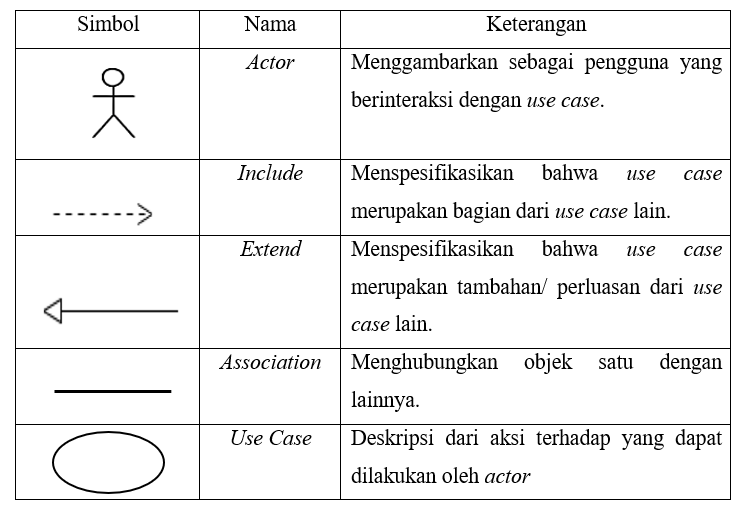
\includegraphics[width=1.0\textwidth]{gambar/simbolusecase}
	\label{tabel_karaktermax2}
\end{table}

\subsection{Diagram \emph{Class}} 

\emph{Class diagram} merupakan salah satu diagram utama dari UML untuk menggambarkan class atau \emph{blueprint object} pada sebuah sistem. Analisis pembentukan \emph{class diagram} merupakan aktivitas inti yang sangat memengaruhi arsitektur piranti lunak yang dirancang hingga ke tahap pengkodean \cite{tanuwijaya}.

%tabel Simbol Class Diagram
\begin{table}[H]
	\centering
	\caption{Simbol-simbol \emph{Class Diagram}}
	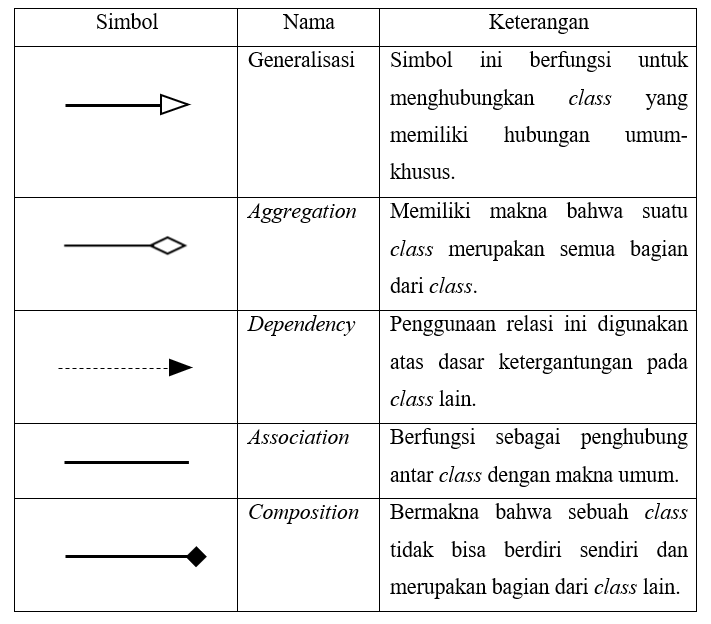
\includegraphics[width=1.0\textwidth]{gambar/simbolclass}
	\label{tabel_karaktermax2}
\end{table}

\subsection{Diagram \emph{Activity}} 

\emph{Activity diagram} menggambarkan berbagai alur kejadian dalam aktivitas sistem yang sedang dalam pengembangan, bagaimana masing-masing alur dimulai, kejadian yang mungkin terjadi, dan bagaimana mereka berakhir. Sebuah aktivitas dapat direalisasikan oleh satu \emph{use case} atau lebih. Aktivitas menggambarkan proses yang berjalan, sementara \emph{use case} menggambarkan bagaimana aktor menggunakan sistem untuk melakukan aktivitas.

%tabel Simbol Activity Diagram
\begin{table}[H]
	\centering
	\caption{Simbol-simbol \emph{Activity Diagram}}
	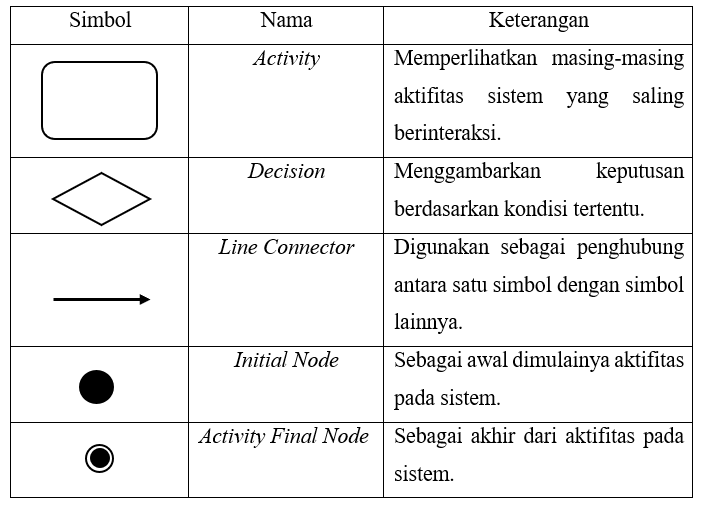
\includegraphics[width=1.0\textwidth]{gambar/simbolactivity}
	\label{tabel_karaktermax2}
\end{table}


\section{\emph{Entity Relationship Database}(ERD)}

ERD merupakan suatu model untuk menjelaskan hubungan antar data dalam \emph{database} berdasarkan objek-objek dasar data yang mempunyai hubungan antar relasi. ERD untuk memodelkan struktur data dan hubungan antar data, untuk menggambarkannya digunakan beberapa notasi dan simbol.

Menurut Brady serta Loonam (2010), \emph{Entity Relationship Diagram} (ERD) adalah suatu teknik yang digunakan untuk dapat memodelkan kebutuhan data dari sebuah organisasi. Biasanya dilakukan oleh \emph{system analys} di dalam tahap analisis persyaratan proyek pengembangan sistem \cite{ibeng}. 

Beberapa jenis relasi antar entitas yang ada pada ERD yaitu \emph{one-to-one}, \emph{one-to-many}, dan \emph{many-to-many}. Dari masing-masing relasi tersebut digunakan tergantung dari kebutuhan data antara entitas yang berhubungan. 

\section{Arsitektur \emph{Model View Controller} (MVC)}

Pola MVC memecah aplikasi menjadi 3 bagian yaitu \emph{model}, \emph{view}, \emph{controller}. Ketiga modul tersebut adalah inti dari aplikasi dan merupakan logika bisnisnya. MVC adalah sebuah konsep yang meng-enkapsulasi basis data, proses manipulasi, dan tampilan untuk direpresentasikan kepada pengguna \cite{simajuntak}. Definisi teknis dari MVC dibagi menjadi tiga bagian.

\subsection{Model}

\emph{Model} digunakan untuk mengolah informasi. Hanya model yang mengandung data dan fungsi yang berhubungan dengan pemrosesan data. Dengan kata lain, model adalah bagian yang mewakili struktur data dalam basis data.

\subsection{View}

\emph{View} adalah bagian yang berfungi dalam pemetaan grafis pada permukaan layar. Ketika ada perubahan dalam \emph{model}, maka \emph{view} akan secara otomatis me-\emph{render} kembali tampilan grafis dan menggambarkannya pada permukaan layar.

\subsection{Controller}

\emph{Controller} dapat disebut juga sebagai jembatan yang menghubungkan antara \emph{model} dan \emph{view}. \emph{Controller} bertanggung jawab dalam memanipulasi proses. Sebagai contoh ketika \emph{user} melakukan perintah \emph{input} maka \emph{controller} akan menentukan bagaimana aplikasi seharusnya merespon.

Secara singkat dapat disimpulkan bahwa \emph{model} bertanggung jawab dalam mengatur alur dari basis data, \emph{view} bertanggung jawab sebagai yang merepresentasikan hasil proses kepada \emph{user} melalui pemetaan pada tampilan layar, dan \emph{controller} bertanggung jawab sebagai penentu respon aplikasi terhadap \emph{input} yang diberikan oleh \emph{user}.

\section{\emph{Framework} Codeigniter} 

Codeigniter (CI) adalah sebuah \emph{framework}/ kerangka kerja aplikasi yang bekerja dibawah \emph{platform} PHP untuk mengembangkan program PHP dengan cara yang lebih sistematis. Codeigniter dikembangkan pertama kali oleh Rick Ellis dan menjadi kerangka kerja yang memiliki lisensi gratis untuk digunakan karena menggunakan lisensi \emph{open-source} apache/BSD dan gratis [7]. \textit{Programmer} tidak perlu melakukan pengembangan dari awal karena telah disediakan beberapa \emph{library} yang dapat digunakan untuk menyelesaikan berbagai permasalahan umum. Codeigniter sendiri menggunakan teknik \emph{Model View Controller} (MVC).

Adapun kelebihan yang dimiliki oleh codeigniter yang menjadi pertimbangan penulis dalam pengembangan penelitian ini antara lain \cite{yicheng} :

\begin{enumerate}
	\item Memiliki ukuran \emph{file} yang relatif kecil.
	\item Mudah dalam proses instalasi. 
	\item Tidak adanya aturan yang terlalu ketat dalam pengkodean.
	\item Mudah untuk migrasi dari satu \emph{server} ke \emph{server} lainnya.
	\item Mudah di-\emph{debug}.
	\item Koleksi \emph{library} yang dimiliki cukup banyak.
	\item Memiliki dokumentasi yang baik sehingga mudah untuk dipelajari.
\end{enumerate}

\section{XAMPP \emph{Server}}

XAMPP adalah sebuah perangkat lunak \emph{web server} Apache yang di dalamnya sudah tersedia \emph{database server} MySQL dan mendukung bahasa pemrograman PHP. XAMPP merupakan singkatan dari X (untuk empat sistem operasi – windows, linux, macOS, dan solaris), Apache, MySQL, PHP, dan Perl \cite{binarso}.

\section{MySQL \emph{Database}}

MySQL merupakan salah satu \emph{software} sistem manajemen \emph{database} bersifat relasional yang disediakan secara gratis di bawah lisensi \emph{General Public License} (GPL). Bahasa SQL adalah bahasa yang menjadi standar bahasa untuk mengakses \emph{database} Oracle, SQL \emph{server}, DB2, dan MySQL \cite{andreea}. Perintah utama SQL terdiri dari lima kategori yaitu bahasa untuk melakukan permintaan, memanipulasi data, mendefinisikan data, kontrol transaksi, dan kontrol data. 

\section{Organisasi Kemahasiswaan Universitas Negeri Jakarta}

Organisasi kemahasiswaan di Univrsitas Negeri Jakarta terbagi atas 2 bagian yaitu Organisasi Pemerintahan Mahasiswa (Opmawa) dan Unit Kegiatan Mahasiswa (UKM). Opmawa adalah organisasi yang berfokus pada kepengtingan birokrasi dan mahasiswa sedangkan UKM adalah organisasi yang berfokus pada minat dan bakat mahasiswa \cite{sartika}.

Organisasi Pemerintahan Mahasiwa (Opmawa) terdiri dari 2 lembaga dan 3 tingkatan yaitu : 
\begin{enumerate}
	\item Tingkat Universitas :
	\begin{enumerate}
		\item Majelis Tinggi Mahasiswa UNJ.
		\item Badan Eksekutif Mahasiswa UNJ.
	\end{enumerate}
	\item Tingkat Fakultas :
	\begin{enumerate}
		\item Badan Perwakilan Mahasiswa Fakultas (BPMF).
		\item Badan Eksekutif Mahasiswa Fakultas (BEMF).
	\end{enumerate} 
	\item Tingkat Program Studi :
	\begin{enumerate}
		\item Badan Legislatif Mahasiswa Prodi (BEMP) / Lembaga Legislatif Mahasiswa Prodi (LLMP).
		\item Badan Eksekutif Mahasiswa Prodi (BEMP) / Himpunan Mahasiswa (Hima).
	\end{enumerate}
\end{enumerate}

Unit Kegiatan Mahasiswa (UKM) terdiri dari 18 organisasi kegiatan mahasiswa yaitu :
\begin{enumerate}
	\item Unit Kesenian Mahasiswa (UKM).
	\item Lembaga Kajian Mahasiswa (LKM).
	\item Unit Keolahragaan Mahasiswa (UKO).
	\item Pramuka Racana.
	\item Komunitas Mahasiswa Pecinta Alam (KMPA).
	\item Korps Sukarela - Palang Merah Indonesia (KSR-PMI).
	\item Kelompok Mahasiswa Peminat Fotografi (KMPF).
	\item Kelompok Sosial Pecinta Anak Universitas Negeri Jakarta (KSPA UNJ).
	\item Resimen Mahasiswa (Menwa).
	\item Badan Penyelenggara Radio Siaran (BPRS) \textit{Educational Radio} (ERAFM-UNJ).
	\item Sinematografi Mahasiswa dan Televisi UNJ (Sigma TV UNJ).
	\item Didaktika.
	\item Koperasi Mahasiswa (Kopma).
	\item Keluarga Mahasiswa dan Alumni Penerima Beasiswa Supersemar (KMA PBS). 
	\item Kelompok Peneliti Muda (KPM).
	\item Lembaga Dakwah Kampus (LDK).
	\item Persekutuan Mahasiswa Kristen (PMK).
	\item Kelompok Mahasiswa Hindu dan Budha.
\end{enumerate} 

\section{Manajemen}

\subsection{Pengertian Manajemen}

Manajemen secara etimologi berasal dari bahasa inggris \emph{management} yang artinya mengatur atau mengelola. Sedangkan di dalam kamus besar bahasa Indonesia kata manajemen memiliki arti sebagai penggunaan sumber daya secara efektif untuk mencapai sasaran. Dalam arti khusus manajemen dipakai oleh pemimpin atau pimpinan yaitu orang-orang yang melakukan kegiatan memimpin di dalam suatu organisasi \cite{syamsuddin}. 

Pada umumnya manajemen dikaitkan dengan kegiatan-kegiatan seperti perencanaan, pengorganisasian, pemberian, pengawasan, pengarahan dan menentukan keputusan. Dari penjelasan di atas dapat disimpulkan bahwa manajemen adalah kegiatan yang berkaitan dengan pengelolaan dengan cara memanfaatkan sumber daya secara efektif melalui beberapa tindakan perencanaan hingga pengambilan keputusan untuk mencapai tujuan dari suatu organisasi.

\subsection{Fungsi Manajemen}

Ada beberapa pendapat menurut para ahli mengenai fungsi dari manajemen adalah sebagai berikut \cite{rifai}: 

%tabel Pengertian Manajemen Menurut Ahli
\begin{table}[H]
	\centering
	\caption{Fungsi manajemen menurut para ahli}
	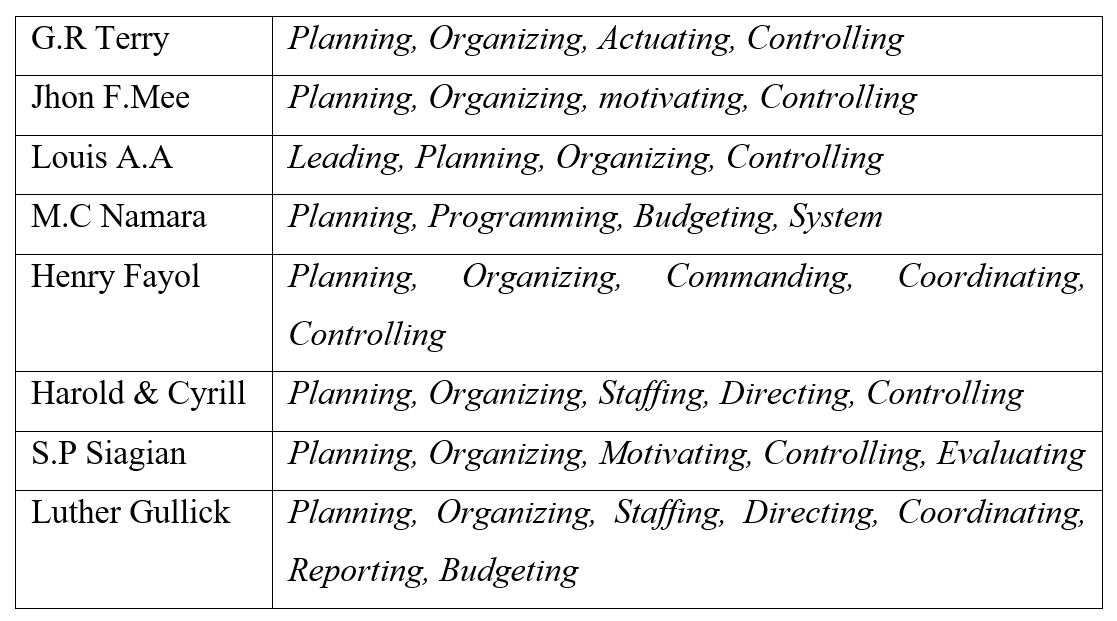
\includegraphics[width=1.0\textwidth]{gambar/manajemenmenurutahli}
	\label{tabel_karaktermax2}
\end{table}

Dari tabel di atas dapat disimpulkan bahwa ada empat fungsi yang menurut penulis penting yaitu perencanaan (\emph{planning}), pengorganisasian (\emph{organizing}), kepemimpinan (\emph{leading}), dan pengaturan (\emph{controlling}). Perencanaan merupakan kegiatan untuk memikirkan langkah kedepan untuk memberikan arah, meminimalisir pengulangan, dan mempermudah pengawasan. Pengorganisasian merupakan kegiatan pembatasan, pengelompokan, dan pemberian tugas kepada sumber daya manusia. Bagi seorang pemimpin organisasi kepemimpinan diperlukan untuk memanajemen sumber daya dan melakukan pengawasan atau pengaturan.

\subsection{Macam-macam Manajemen}

Manajemen dapat diterapkan di dalam berbagai bentuk organisasi. Setiap organisasi memiliki norma dan aturan sendiri dalam menerapkan manajemen sebagai sistem yang menjalankan roda organisasi. Menurut Made Pidarta, sebuah sistem manajemen dapat dilihat dari berbagai sudut pandang berikut \cite{athhoillah} :

\begin{enumerate}
	\item \emph{Management by objective} \\*
	Dalam manajemen sasaran, seluruh elemen diintegrasikan dan ditargetkan kepada sasaran atau tujuan yang telah ditentukan. Biasanya dalam organisasi memiliki tiga tingkatan, yaitu tujuan jangka pendek, tujuan jangka menengah, dan tujuan jangka panjang. Manajemen berdasarkan sasaran sangat mementingkan adaptabilitas semua subsistem dan komponen di dalamnya. Dalam pelaksanaan rencana kegiatan interaktif adaptif antara tujuan dan seluruh sumber daya. Dengan demikian seluruh komponen di dalam organisasi harus memiliki ikatan yang kuat untuk mewujudkan tujuannya. 
	
	\item \emph{Management by structures} \\*
	Manajemen dengan pendekatan struktural berawal dari pandangan bahwa organisasi adalah struktur yang harus dikelola secara struktural. Oleh karena itu pelaksanaan manajerial berdasarkan kedudukan, peran, dan tugas setiap personalia dalam strukturnya masing-masing.
	
	\item \emph{Management by technique} \\*
	Dalam manajemen Teknik, penguasaan terhadap Teknik-teknik pelaksanaan kegiatan lebih diutamakan. Sebagai contoh, sebuah organisasi menginginkan sebuah acara yang menggabungkan suasana tradisional namun tetap bernuansa modern. Hal-hal yang dibahas lebih tertuju kepada bagaimana cara perpaduan yang dimaksud, apa saja alat yang diperlukan, berapa biayanya, dan hal-hal teknis lainnya.
	
	\item \emph{Management by people} \\*
	Manajemen ini mengutamakan sumber daya manusia sebagai pelaksana seluruh rencana organisasi. Orang-orang yang terlibat disebut sebagai personalia. Dalam manajemen personalia, seorang pimpinan tertinggi tidak hanya terpaku pada hubungan vertikal kekuasaan struktural, tetapi perlu juga membangun hubungan yang interaktif dengan seluruh bawahannya.
	
	\item \emph{Management by information} \\*
	Manajemen dengan pendekatan informasi adalah pengelolaan organisasi yang berpusat pada peran pentingnya informasi bagi kemajuan dan kinerja organisasi. Informasi merupakan media yang menciptakan relasi maupun sebagai data untuk mengetahui keadaan organisasi yang sesungguhnya. Informasi bukan hanya menjadi sebuah berita, melainkan tentang berbagai kondisi internal maupun eksternal organisasi.
	
	\item \emph{Management by environment} \\*
	Lingkungan organisasi adalah segala sesuatu yang ada di sekeliling organisasi. Faktor internal dan eksternal seperti manusia, fasilitas, sarana, transportasi dan lain-lain. Lingkungan yang sangat menentukan kemajuan organisasi adalah lingkungan masyarakat karena organisasi mengadakan kontak secara langsung dengan masyarakat. Contohnya, pertokoan yang dekat dengan organisasi akan lebih memudahkan organisasi dalam memeroleh barang yang dibutuhkan.
\end{enumerate}

\section{Program Kerja}

Program kerja adalah sebuah susunan rencana kegiatan yang telah dirancang dan disepakati bersama oleh anggota/ pengurus organisasi untuk dilaksanakan dalam jangka waktu tertentu. Program kerja bertujuan sebagai media untuk merealisasikan visi dan misi dari organisasi, membantu menjawab kebutuhan organisasi baik dari segi internal maupun eksternal, dan membantu organisasi bekerja secara sistematis dan terstruktur \cite{dosen}.

Program kerja yang ada di opmawa pada umumnya terdiri dari dua jenis program kerja yaitu program kerja yang bersifat \emph{event} dan program kerja yang bersifat \emph{non-event}. Program kerja \emph{event} merupakan kegiatan yang melibatkan masyarakat umum di dalam pelaksanaannya. Contoh dari program kerja  yang bersifat \emph{event} antara lain berupa seminar, \emph{workshop}, dan sebagainya. Sedangkan program kerja \emph{non-event} biasanya hanya bersifat internal dalam organisasi untuk meningkatkan kebersamaan dan kemampuan berorganisasi.

Adapun tahapan-tahapan dalam pelaksanaan program kerja secara umum antara lain yaitu studi kasus permasalahan dan kebutuhan, perencanaan kegiatan, pelaksanaan, dan evaluasi.

%\section{Penelitian Relevan}
%Beberapa hasil penelitian mengenai sistem informasi manajemen yang relevan sebelumnya dengan penelitian ini antara lain:

%\begin{enumerate}[A.]
%	\item Penelitian yang dilakukan oleh Yogi Perdana pada tahun 2019 dalam skripsinya yang berjudul “Perancangan dan Implementasi Aplikasi Penilaian Kinerja Badan Eksekutif Mahasiswa Universitas Negeri Jakarta Berbasis \emph{Web}”. Model pengembangan perangkat lunak yang digunakan adalah dengan menggunakan model Spiral. Penelitian tersebut bertujuan untuk memberikan penilaian terhadap kinerja Badan Eksekutif Mahasiswa (BEM) melalui instrumen penilaian yang telah ditetapkan oleh Badan Legislatif Mahasiswa atau biasa disebut sebagai Majelis Tinggi Mahasiswa (MTM) terhadap program kerja BEM yang telah terlaksana. Sistem tersebut memungkinkan MTM untuk mengelola instrumen penilaian sebagai acuan untuk penilaian kinerja BEM dengan cara membuat indikator penilaian beserta bobot untuk setiap indikatornya. Setelah instrumen penilaian telah ditetapkan, maka komisi yang berkaitan memberikan penilaian terhadap program kerja BEM sesuai dengan interval bobot untuk setiap indikator penilaian \cite{perdana}.
	
%	Persamaan penelitian tersebut dengan penelitian yang akan penulis lakukan adalah sama-sama berkaitan dengan program kerja yang di lakukan oleh BEM. Model pengembangan yang digunakan sama-sama menggunakan model Spiral dan menggunakan \emph{framework} yang sama yaitu Codeigniter. Pada penelitian ini, sistem yang akan dibangun juga dapat memberikan penilaian terhadap program kerja BEM yang telah terlaksana.
	
%	Perbedaannya dalam penelitian tersebut dengan penelitian yang akan penulis lakukan terletak pada fokus dan tingkatan opmawa. Penelitian tersebut terfokus pada pembuatan instrumen penilaian, sedangkan penelitian yang akan penulis lakukan terfokus pada proses manajemen program kerja dari awal terencananya program kerja hingga program kerja tersebut selesai terlaksana. Pada penelitian ini juga memungkinkan sebagai jembatan informasi antar lintas lembaga dan lintas periode kepengurusan opmawa. Pada penelitian tersebut bertujuan untuk opmawa pada tingkat Universitas sedangkan penelitian ini berada pada opmawa tingkat Fakultas.
	
%	\item Penelitian yang dilakukan oleh Muhammad Yan Handoko pada tahun 2019 dalam skripsinya yang berjudul "Perancangan Sistem Informasi Koperasi Serba Usaha Berbasis \textit{Website} Pada Lembaga Koperasi Mahasiswa Universitas Negeri Jakarta". Model pengembangan perangkat lunak yang digunakan adalah dengan menggunakan model Spiral. Penelitian tersebut bertujuan untuk membangun sistem informasi yang dapat mempermudah pengolahan data baik itu pengolahan data anggota, simpanan, usaha, dan pendistribusian sisa hasil usaha \cite{handoko}. 
	
%	Persamaan penelitian tersebut dengan penelitian yang akan penulis lakukan adalah sama-sama berkaitan dengan fungsi manajerial organisasi dalam menjalankan program kerjanya dan menggunakan model pengembangan Spiral. Kedua sistem juga dikembangkan menggunakan \textit{framework} yang sama.
	
%	Perbedaannya dalam penelitian tersebut dengan penelitian yang akan penulis lakukan terletak pada organisasi yang menjadi objek penelitian dan perbedaan program kerja yang dilaksanakan oleh masing-masing organisasi.
	
%	\item Penelitian yang dilakukan oleh La Ode Ismail Ahmad dan Ristati Sinen dalam jurnal Idaarah Vol.I No.2 Desember 2017 menjelaskan tentang penerapan sistem informasi manajemen pada SMPN 21 Makassar. Penggunaan sistem informasi manajemen pada dunia pendidikan diperlukan guna meningkatkan efesiensi dalam kegiatan belajar mengajar dan memberikan kesempatan kepada guru dan pengurus sekolah untuk meningkatkan kualitas komunikasi dan pembinaan kepada siswa \cite{ahmad}.
	
%	Persamaan penelitian tersebut dengan penelitian yang akan penulis lakukan adalah pemanfaatan sistem informasi manajemen dalam pengolahan data untuk diolah menjadi sebuah informasi yang berguna dalam pengambilan keputusan manajerial. Sistem yang akan dirancang oleh penulis memiliki tujuan yang sama dengan sistem informasi manajemen yang ada pada SMPN 21 Makassar. 
 
% 	Perbedaannya dalam penelitian tersebut dengan penelitian yang akan penulis lakukan terletak pada objek organisasi dan pokok pembahasan yang diteliti.
 	
% 	\item Penelitian yang dilakukan oleh Etin Indrayani dalam \textit{Journal of Social Sciences Research} Vol.9 No.3 Desember 2015 menjelaskan tentang pengimplementasian sistem informasi manajemen pada pelayanan administrasi kecamatan Sragen. Pada penelitian tersebut membahas mengenai penggunaan sistem informasi manajemen dalam mengoperasikan fungsional organisasi \cite{indrayani}.
 	
% 	Persamaan penelitian tersebut dengan penelitian yang akan penulis lakukan adalah pembahasan mengenai pemanfaatan sistem informasi manajemen dalam pengelolaan fungsional organisasi. Pengelolaan terkait pada permasalahan anggaran, keanggotaan, penyebaran informasi, interaksi organisasi eksekutif, dan lain-lain.
 	
% 	Perbedaannya dalam penelitian tersebut dengan penelitian yang akan penulis lakukan terletak pada objek organisasi dan pokok pembahasan yang diteliti.
	
	
%\end{enumerate}
		
% Baris ini digunakan untuk membantu dalam melakukan sitasi
% Karena diapit dengan comment, maka baris ini akan diabaikan
% oleh compiler LaTeX.
\begin{comment}
bibliography{daftar-pustaka}
\end{comment}
